\providecommand{\StudySection}{\section}
\providecommand{\StudySubsection}{\subsection}

\StudySection{Testing integral and propagator orderings}
\label{sec:ordering-policy}
Selective seed expansion reduces equation-generation work, but the ordering of the resulting integrals can still affect elimination. Kira provides eight integral priority rules and four automatic propagator-ordering schemes~\cite{Kira12,Kira3}. We test whether a model can choose among these settings from the target indices before equation generation, while retaining the seed strategy from Section~\ref{sec:basis-completion}. The model makes one decision for each batch, and a failed basis check triggers a repeat with the preceding settings. Appendix~\ref{app:ordering-policy} defines the candidates and shows why consistent relabelling preserves the integrals.

Development first compares eleven candidates and then tests the pair of best nondefault orderings for each batch. We keep the preceding settings and any batch winner that saves at least ten percent of complete time. If $\omega$ is the integral-order number and $\chi$ the propagator-scheme number, the retained new settings are $(\omega,\chi)=(2,1)$, $(7,1)$, $(5,4)$, and $(8,3)$. The preceding method also remains available without a change in its settings.

We fit ten predictors per graph on 36 training batches, select their use on 18 validation batches, and test on 36 reserved batches. The features, complete-time labels, candidate model types, and five-percent validation requirement are the same as in the seed-expansion study. A fixed ordering still uses the preceding learned seed strategy, so the fixed-setting comparison measures the additional ordering decision. Training and validation contain 1,432.8 seconds of reductions, and fitting the seventy predictors takes 0.93 seconds. These offline costs exclude development and reference construction.

None of the predictors passes the validation requirement. The tested selected method therefore uses fixed ordering settings chosen by validation, with no newly enabled ordering predictor. Any difference in its time reflects those settings, their interaction with the retained seed strategy, and execution variation. This distinction is necessary when interpreting the results as evidence about machine learning.

All 720 timed reductions and 43 additional applications pass exact checks; the additional applications receive no target reference coefficients during reduction. With equal weight for each graph, the selected-to-preceding ratio is $1.0141$ with descriptive interval $[0.9986,1.0303]$, giving 1.4\% more time. The selected-to-native ratio is $0.8499$ with interval $[0.7306,0.9642]$, giving 15.0\% less time, while the ratio to the new fixed strategy is $1.0070$ with interval $[0.9811,1.0327]$. The saving against native choices therefore does not show an improvement over the already learned seed-expansion method.

The sum of median times over the 36 test batches is 110.09 seconds for native choices, 79.61 seconds for the preceding method, 79.53 seconds for the new fixed settings, and 79.68 seconds for the selected settings. On this workload, the selected method takes 0.1\% more time than its predecessor. Its additional ordering decision takes a median of 271.1 microseconds per application, and both this cost and the retained seed-policy cost are included in complete time.

\begin{table}[!htbp]
\centering\small
\caption{Ordering settings compared with the seed-expansion method in Section~\ref{sec:basis-completion}. Times are geometric means of batch medians in seconds. ``Previous'' retains the earlier ordering, and ``New'' uses the selected setting. The pair $(\omega,\chi)$ specifies the integral order and propagator scheme.}
\label{tab:ordering-policy}
\begin{tabular}{@{}llrrrr@{}}\toprule
Graph & Choice & Previous (s) & New (s) & New/previous & New/native\\\midrule
Sunrise & $(7,1)$ & 0.610 & 0.633 & 1.037 & 1.034\\
Planar box & $(2,1)$ & 2.407 & 2.390 & 0.993 & 0.759\\
Vacuum & Previous & 0.975 & 0.982 & 1.007 & 0.983\\
Ladder & Previous & 3.122 & 3.088 & 0.989 & 0.591\\
Nonplanar box & $(2,1)$ & 3.698 & 3.681 & 0.995 & 0.745\\
Pentagon & $(2,1)$ & 0.788 & 0.820 & 1.041 & 0.987\\
Virtuality box & $(5,4)$ & 0.601 & 0.624 & 1.039 & 0.955\\
\bottomrule\end{tabular}
\end{table}

\begin{figure}[!htbp]
\centering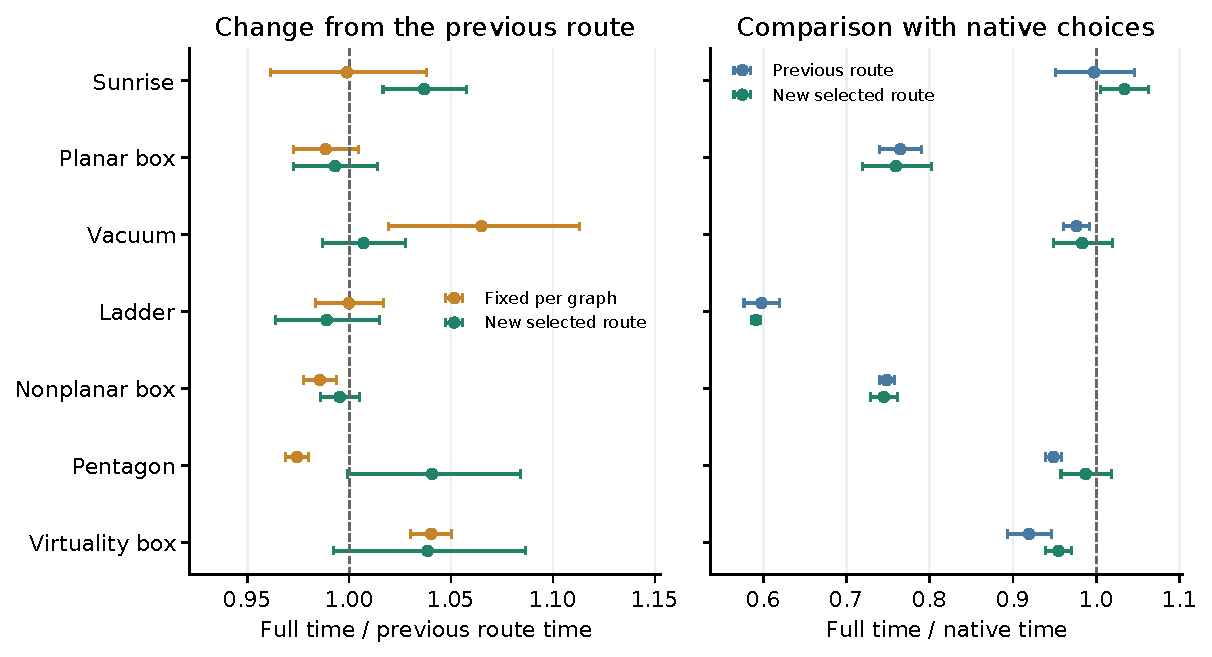
\includegraphics[width=\linewidth]{paper_figures/ordering_policy.pdf}
\caption{The effect of choosing Kira settings before reduction. Left:
new fixed settings and selected settings relative to the preceding method.
Right: preceding and selected methods relative to native choices.
Values below one indicate less complete time. Bars give the range across
two parameter profiles; they are not significance intervals.}
\label{fig:ordering-policy}
\end{figure}

\FloatBarrier

The sunrise, vacuum, pentagon, and box with external virtuality take 3.7\%, 0.7\%, 4.1\%, and 3.9\% more time, respectively. No selected calculation requires fallback. Across 180 runs per method, symbolic equation regeneration changes from 79.88 to 80.58 seconds, while back-substitution changes from 37.99 to 37.35 seconds. These stage measurements show small changes in opposite directions rather than a consistent overall improvement.

The timers include prediction, preparation, native generation, exact checks, basis conversion, retries, and cleanup. As in the preceding comparisons, the caller and models are already loaded, and each attempt starts a fresh Kira process. The evidence therefore supports retaining the earlier ordering for this measured workload of known one- through three-loop graphs at new rational parameter values. The next comparison keeps that choice and changes the amount of parallel work instead.
